\documentclass[12pt,letterpaper]{article}
\usepackage[latin1]{inputenc}
\usepackage{amsmath}
\usepackage{amsfonts}
\usepackage{amssymb}
\usepackage{graphicx}

\newtheorem{clm}{Claim}

\author{Linyun Fu}
\title{CSCI 4020 Computer Algorithms Spring 2011\\
Programming Assignment \#1}
\begin{document}
\maketitle
\section*{Chapter 4, Problem 7}
The wildly popular Spanish-language search engine El Goog needs to do
a serious amount of computation every time it recompiles its index. Fortunately,
the company has at its disposal a single large supercomputer,
together with an essentially unlimited supply of high-end PCs.

They've broken the overall computation into $n$ distinct jobs, labeled
$J_1, J_2, ..., J_n$, which can be performed completely Independently of one
another. Each job consists of two stages: first it needs to be preprocessed
on the supercomputer, and then it needs to be finished on one of the
PCs. Let's say that job $J_i$ needs $p_i$ seconds of time on the supercomputer,
followed by $f_i$ seconds of time on a PC.

Since there are at least $n$ PCs available on the premises, the finishing
of the jobs can be performed fully in parallel -- all the jobs can be processed
at the same time. However, the supercomputer can only work on
a single job at a time, so the system managers need to work out an order
in which to feed the jobs to the supercomputer. As soon as the first job
in order is done on the supercomputer, it can be handed off to a PC for
finishing; at that point in time a second job can be fed to the supercomputer;
when the second job is done on the supercomputer, it can proceed
to a PC regardless of whether or not the first job is done (since the PCs
work in parallel); and so on.

Let's say that a schedule is an ordering of the jobs for the supercomputer,
and the completion time of the schedule is the earliest time at
which all jobs will have finished processing on the PCs. This is an important
quantity to minimize, since it determines how rapidly El Goog can
generate a new index.

Give a polynomial-time algorithm that finds a schedule with as small
a completion time as possible.

\section*{Answer}
The algorithm is sorting the job in decreasing order of their PC times ($f_i$), and schedule them in this order. Sorting $n$ numbers costs $O(n\log n)$ running time, which is the time complexity of this algorithm.

To simplify the proof of the correctness of this algorithm, we rename the jobs so that 
\begin{align}
f_1 \ge f_2 \ge ... \ge f_n
\end{align}
We say that a schedule has an \emph{inversion} if a job $i$ is scheduled before another job $j$, but $f_i < f_j$.

\begin{clm}
In a schedule without inversions, the order of the jobs with the same PC time does not affect the completion time.
\end{clm}
\textbf{Proof} Since there is no inversion in the schedule, jobs with the same PC time must stay together as consecutive jobs. Among the jobs with PC time $f$, the last one is the last to finish, and its finishing time is not affected by the order of the jobs.

\begin{clm}
In a schedule with an inversion, there must be two adjacent jobs $i$ and $j$ such that $f_i < f_j$.
\end{clm}
This claim has been proved during the class.

Starting from an optimal schedule, if there is any inversion in it, from Claim~2 we know that there must be two adjacent jobs $i$ and $j$ such that $f_i < f_j$. We now prove that swapping $i$ and $j$ does not make the schedule worse.

\begin{figure}
\begin{center}
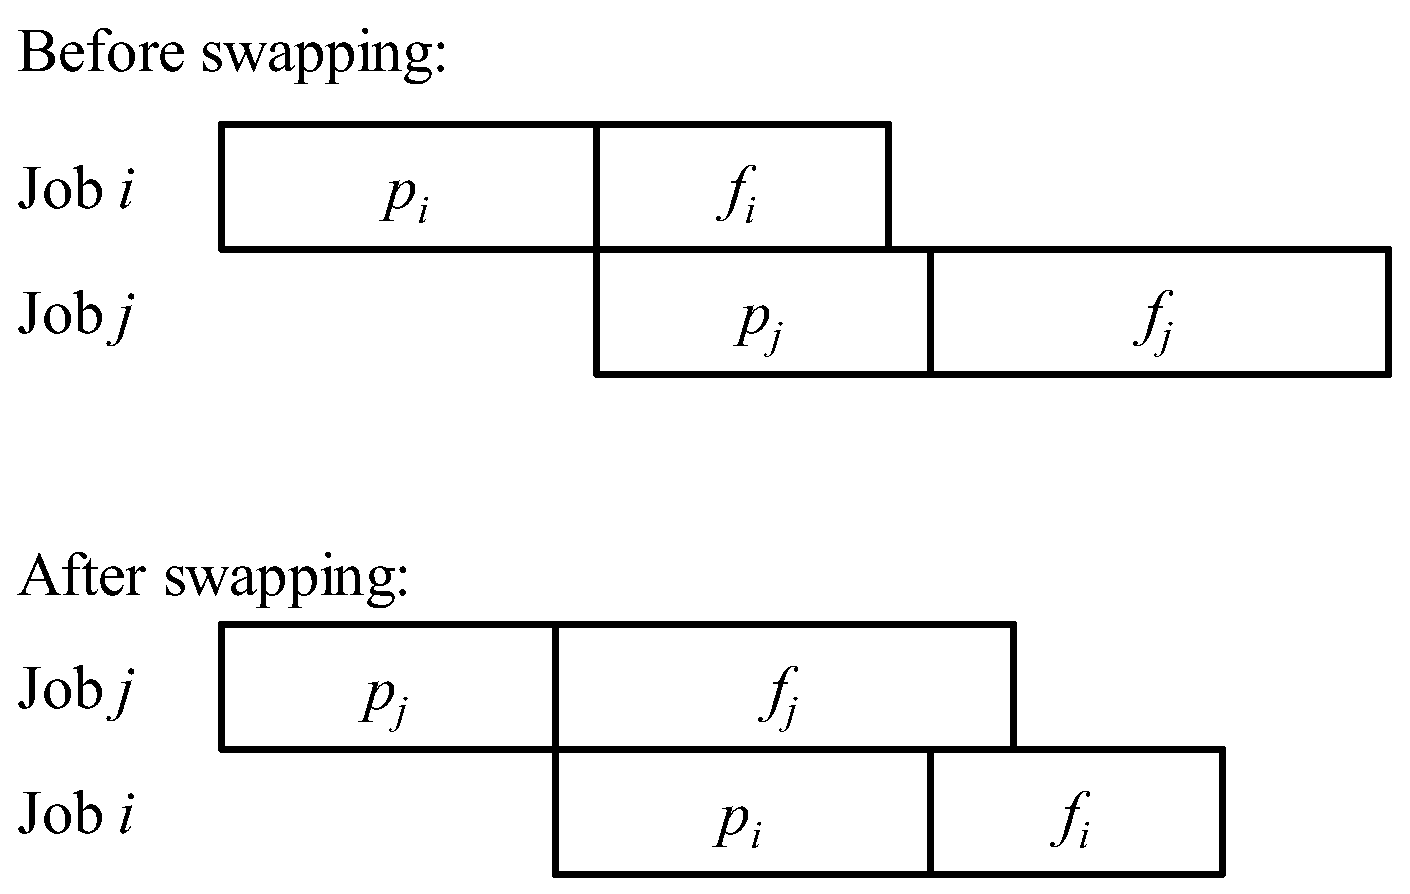
\includegraphics[width=0.7\textwidth]{4.7.eps}
\caption{The effect of swapping two adjacent inverted jobs}
\end{center}
\end{figure}
Figure~1 roughly pictures the swapping effect. We denote the finishing time of job $r$ as $d_r$ before swapping and $\bar{d_r}$ after swapping, then the completion time before swapping is $C=\max_r{d_r}$ and is $\bar{C}=\max_r{\bar{d_r}}$ after swapping. We can see that the finishing times are not changed by the swapping for all the jobs except $i$ and $j$, and we have
\begin{align}
\bar{d_j}-d_j = -p_i < 0
\end{align}
and
\begin{align}
\bar{d_i}-d_j = p_j+p_i+f_i-(p_i+p_j+f_j) = f_i - f_j < 0
\end{align}
This means both job $i$ and job $j$ finishes before $d_j$ (thus before $C$) after swapping. Since the finishing times for all the other jobs do not change with the swapping, it is true that $\bar{C}\le C$, which completes the proof.

\section*{Chapter 4, Problem 14}
You're working with a group of security consultants who are helping to
monitor a large computer system. There's particular interest in keeping
track of processes that are labeled ``sensitive.'' Each such process has a
designated start time and finish time, and it runs continuously between
these times; the consultants have a list of the planned start and finish
times of all sensitive processes that will be run that day.

As a simple first step, they've written a program called \texttt{status\_check}
that, when invoked, runs for a few seconds and records various pieces
of logging information about all the sensitive processes running on the
system at that moment. (We'll model each invocation of \texttt{status\_check}
as lasting for only this single point in time.) What they'd like to do is to
run \texttt{status\_check} as few times as possible during the day, but enough
that for each sensitive process $P$, \texttt{status\_check} is invoked at least once
during the execution of process $P$.

\begin{itemize}
\item[(a)] Give an efficient algorithm that, given the start and finish times of
all the sensitive processes, finds as small a set of times as possible
at which to invoke \texttt{status\_check}, subject to the requirement
that \texttt{status\_check} is invoked at least once during each sensitive
process $P$.
\item[(b)] While you were designing your algorithm, the security consultants
were engaging in a little back-of-the-envelope reasoning. ``Suppose
we can find a set of $k$ sensitive processes with the property that no
two are ever running at the same time. Then clearly your algorithm
will need to invoke \texttt{status\_check} at least $k$ times: no one invocation
of \texttt{status\_check} can handle more than one of these processes.''

This is true, of course, and after some further discussion, you all
begin wondering whether something stronger is true as well, a kind
of converse to the above argument. Suppose that $k^*$ is the largest
value of $k$ such that one can find a set of $k$ sensitive processes with
no two ever running at the same time. Is it the case that there must
be a set of $k^*$ times at which you can run \texttt{status\_check} so that some
invocation occurs during the execution of each sensitive process? (In
other words, the kind of argument in the previous paragraph is really
the only thing forcing you to need a lot of invocations of
\texttt{status\_check}.) Decide whether you think this claim is true or false, and give
a proof or a counterexample.
\end{itemize}

\section*{Answer}
\subsection*{Problem (a)}
Let us denote the number of sensitive processes that need to be checked as $n$, the start time of process $i$ as $s_i$ and the finish time of process $i$ as $f_i$. 

The algorithm works in the following way. First, we sort all the processes in increasing order of their finish times, and label all of them \texttt{un-eliminated}, then we pick the process with the earliest finish time from among the un-eliminated ones, invoke a \texttt{status\_check} operation at its finish time $f$, and label all the processes with start times earlier than $f$ as \texttt{eliminated}. Let us call the picked processes \emph{key processes}, denoted as $K$. We pick processes one by one in this way until all the processes are labeled \texttt{eliminated}, the number of invocations of \texttt{status\_check} is the size of set $K$.

Note that if at some point there are two or more processes having the same earliest finish time, we can pick any of them without influencing the result. 

Sorting $n$ processes according to their finish times takes $O(n\log n)$ time, and we can also sort these processes in increasing order of their start times to facilitate elimination, which also takes $O(n\log n)$ time, then all the eliminations can be carried out by a one-pass scanning of all the sorted processes, which takes $O(n)$ time in all. So the time complexity of this algorithm is $O(n\log n)$.

To simplify the proof of the correctness of these algorithm, let us rename the processes so that $f_1 \le f_2 \le ... \le f_n$.

Consider an optimal invocation scheme $OPT$, since each process must be checked at least once during its life cycle, $OPT$ must invoke \texttt{status\_check} at least once between the start time and finish time of each key process in $K$.

Let $p_1$ be the earliest key process that has a \texttt{status\_check} in its middle in $OPT$, we try to prove that postponing the \texttt{status\_check} to the finish time of $p_1$ will not make any process miss its \texttt{status\_check}.

Suppose when we postpone the \texttt{status\_check}, another process $p_2$ misses its \texttt{status\_check}, then the whole life cycle of $p_2$ must be either to the left or to the right of the finish time of $p_1$. Since we only change one \texttt{status\_check}, $p_2$ must be originally checked by this \texttt{status\_check}, so $p_2$ finishes before $p_1$, as shown in Figure~2.

\begin{figure}
\begin{center}
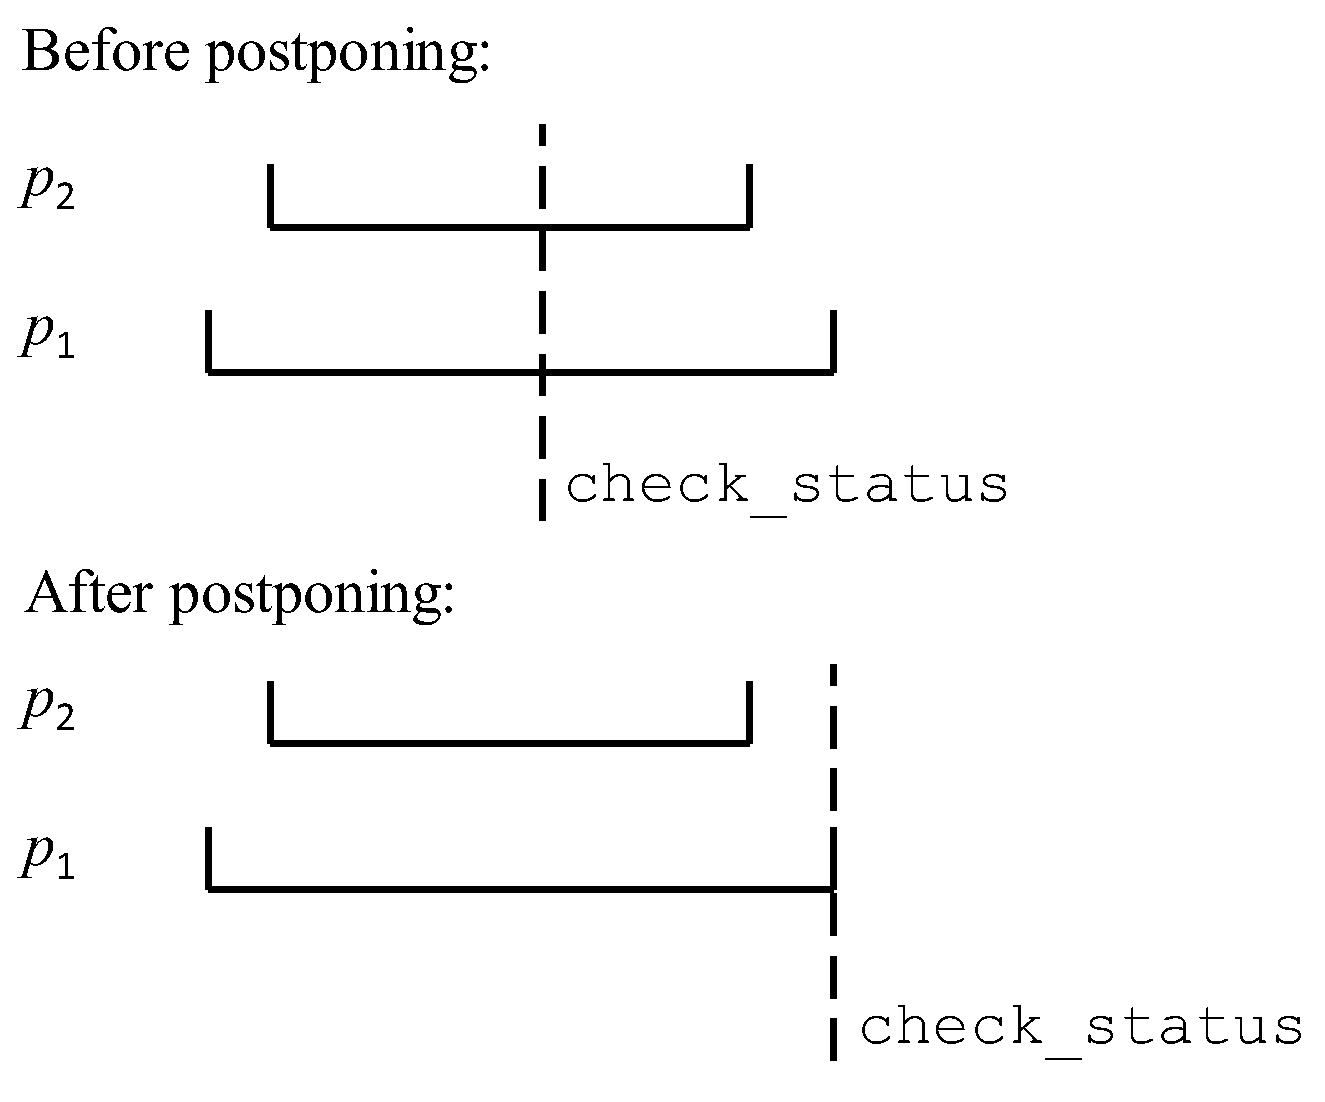
\includegraphics[width=0.7\textwidth]{4.14.eps}
\caption{Hypothetical influence of postponing a \texttt{check\_status}}
\end{center}
\end{figure}

But according to the definition of key processes, at the time we pick $p_1$ as a key process, $p_2$ must either have been \texttt{eliminated} or has a later finish time than $p_1$, so the situation shown in Figure~2 cannot exist.

Starting from $OPT$, we can pick the key processes one by one, from the earliest to the latest, and postpone the \texttt{check\_status}'s in the middle of each key process to its finish time, thus arriving at the result of our proposed algorithm. Since we do not add any \texttt{check\_status} during the whole process, the final result does not contain more \texttt{check\_status}'s than $OPT$. This proves that the proposed algorithm can achieve the optimal result.

\subsection*{Problem (b)}
We try to prove the truth of the claim, i.e., 
\begin{quote}
suppose that $k^*$ is the largest
value of $k$ such that one can find a set of $k$ sensitive processes with
no two ever running at the same time, then there must
be a set of $k^*$ times at which you can run \texttt{status\_check} so that some
invocation occurs during the execution of each sensitive process. 
\end{quote}

Since the choosing strategy guarantees that no two key processes ever running at the same time, and invoking \texttt{check\_status} at the finish time of each key process guarantees each process being checked during its execution, the only thing we need to prove now is that the number of key processes $|K|$ equals $k^*$, i.e., no set of non-overlapping processes has size larger than $|K|$.

Consider the $|K|$ \texttt{check\_status}'s at the finish times of the key processes, they check all the processes. For any set of processes with size larger than $|K|$, it must contain two processes checked by the same \texttt{check\_status}, which means they are both running at the time of the \texttt{check\_status}. So the largest set of non-overlapping processes must contain no more than $|K|$ processes. This completes the proof.
\end{document}

